\chapter{Verwandte Arbeiten}
Die Idee für interaktive Türschilder wurde schon in verschiedenen wissenschaftlichen Ausarbeitungen sowie in der Praxis erarbeitet.
Die Gruppe um Keith Cheverest et al. von der Universität Lancaster hat mehrere Paper für ihr Türschild-System ``Hermes''\cite{cheverest:2003:paper} bereits ab 2003 veröffentlicht.
Das Projekt ``NetBoards'' von Errol Wood\cite{wood:2014} von der Universität Cambridge behandelt eine aktuellere Version interaktiver Türschilder.
Zudem gab es noch einige andere Arbeiten, die sich mit ähnlichen Ansätzen befassten und teilweise als Grundlage für diese beiden Projekte dienten.

\section{Hermes}
Das Hermes System\cite{cheverest:2003:paper,cheverest:2003:article,cheveres:2005:hermes-bluetooth} ist eines der ersten Versionen interaktiver digitaler Türschilder im Bürobereich.
Es diente dazu herauszufinden, ob die \quelle{traditionelle Methode Nachrichten in einem halbwegs öffentlichem Raum (wie \bspw vor Büros in einem Forschungsinstitut) mittels Post-It-Zetteln zu hinterlassen durch eine digitale Methode verbessert werden könnte}{cheverest:2003:paper,cheverest:2003:article}.
Zu diesem Zweck haben die Forscher ein digitales asynchrones Nachrichtensystem entwickelt, welches direkte Interaktion mittels eines vor den Büros angebrachten Interfaces, sowie Fernzugriff durch ein Web-Portal und SMS ermöglicht.
Das System bestand aus einem Web-Server und mehreren PDA's, welche an die Wände neben den Büroeingängen angebracht wurden \abb{img:hermesDisplay}.
\begin{figure}[h!]
  \centering
  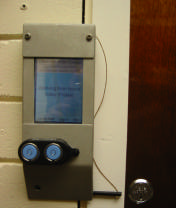
\includegraphics[width=0.5\textwidth]{./img/hermes_display.png}
  \caption{Das erste Hermes Display\cite{cheverest:2003:paper}}
  \label{img:hermesDisplay}
\end{figure}
Der Server wurde mit Java-Servlets realisiert und generierte HTML Webseiten, die auf den Displays angezeigt werden. Er bot eine zentrale Datenbank für alle Daten des Systems und diente als Kommunikationseinheit mit einem SMS-Gateway.
Eines der Hauptblickpunkte von Hermes war, dass das System leicht einsetzbar ist. Deswegen fiel die Entscheidung zur Wahl der Geräte auf PDA's. Zu der Zeit, als das Paper entstand, waren PDA's die beste Wahl für kleine, handliche Geräte, welche per WLAN mit einem Server kommunizieren konnten. Zudem mussten die Geräte mit der Umweltpolitik der Universität übereinstimmen und sollten daher nicht viel Energie verbrauchen.
Um die Geräte vor Diebstahl zu schützen, wurden Aluminiumhüllen für die PDA's entworfen, welche neben den Büroeingängen an die Wand geschraubt werden konnten und zudem auch als Diebstahlsicherung dienten. Um unerwünschte Interaktion zu verhindern, wurden die Hüllen so konzipiert, dass die Tasten nicht direkt zugänglich waren.
\\
Die Funktionen von Hermes wurden in zwei Perspektiven aufgeteilt: Die Besitzerperspektive und die Besucherperspektive.
\\\todotext{fußnote für was ist ein gif machen}
\subsubsection{Besitzerperspektive}
\quelle{Diese Perspektive ermöglicht dem Besitzer des Displays entweder Nachrichten oder Bilder zu erstellen, die dann direkt auf dem PDA angezeigt werden oder Nachrichten zu lesen, die von Gästen für ihn hinterlassen wurden}{cheverest:2003:paper}. Zudem kann der Nutzer animierte Gifs hochladen.
Der Nutzer kann die Perspektive von einem PC oder direkt am Display aufrufen, was ihm ermöglicht, schnell beim Verlassen des Büros eine Nachricht zu schreiben. Um sich zu authentisieren, muss er entweder seinen Nutzernamen und sein Passwort eingeben oder sich mit seinem iButton\footnote{Ein iButton ist ein Mikrochip in einer Metallhülle und dient \bspw zum Authentisieren des Besitzers \cite{iButton:website}} anmelden.
\subsubsection{Besucherperspektive}
\quelle{Besucher müssen sich vor dem PDA befinden, um mit dem System interagieren zu können}{cheverest:2003:paper}. Sie können dem Besitzer des Raumes Nachrichten schreiben. Andere Besucher können jedoch nur die Nachricht sehen, die der Besitzer des Raumes eingestellt hat. Die Nachrichten von anderen Besuchern kann nur der Besitzer einsehen, wodurch ein Vorteil im Bereich der Privatsphäre gegenüber Post-It-Zetteln erzielt wurde.
\\
\\
Um das System zu testen haben die Entwickler eine Langzeitstudie über 15 Monate durchgeführt. Dabei haben sie im Vorfeld Bedenken geäußert, dass \quelle{die Nutzer Zeit brauchen bis sie neue Technologien in ihre tägliche Routine eingliedern}{cheverest:2003:paper}.
Eines der enttäuschensten Ergebnisse war, dass es Nutzer gab, die trotz aufgehängtem Hermes Display weiterhin Post-Its an die Türen geklebt haben\cite{cheverest:2003:paper}.
Ein weiteres Ergebnis der Studie war, dass die Nutzer erst Vertrauen aufbauen mussten. \quelle{Nutzer gebrauchen ein neues System erst, wenn sie wissen, dass es funktioniert}{cheverest:2003:paper}. Durch Verbindungsprobleme über das WLAN kam es dazu, dass das System ab und an nicht reagierte, wodurch es für die Nutzer schien, das Gerät wäre abgestürzt. Um dies zu beheben, wurde das Metallgehäuse an der Stelle des WLAN Adapters geöffnet, damit das Gehäuse das Signal nicht weiter abschwächen konnte.
Es kam auch vor, dass Besucher vergaßen ihre Nachricht abzuschicken, wodurch deren Nachricht nicht mehr privat war und andere Nutzer sie sehen konnten. Das ermöglichte anderen Nutzern die Nachricht zu verändern oder sie zu missbrauchen um unangebrachte Nachrichten zu schreiben. Wenn der eigentliche Benutzer sich zudem auch authentisiert hat wurde die Nachricht dann in seinem Namen geschickt\cite{cheverest:2003:article}.
Manche Nutzer fanden es frustrierend, nachdem sie eine temporäre Mitteilung eingestellt hatten, eine alte Nachricht wiederherzustellen, da sie wieder durch den Prozess einer neuen Mitteilung gehen mussten. Als Lösung dafür wurde eine Möglichkeit eingebaut, mit der die Nutzer eine Standardnachricht einstellen konnten, die nach Entfernen der temporären Nachricht wieder angezeigt wurde\cite{cheverest:2003:article}.
\\
\begin{figure}[h!]
  \centering
  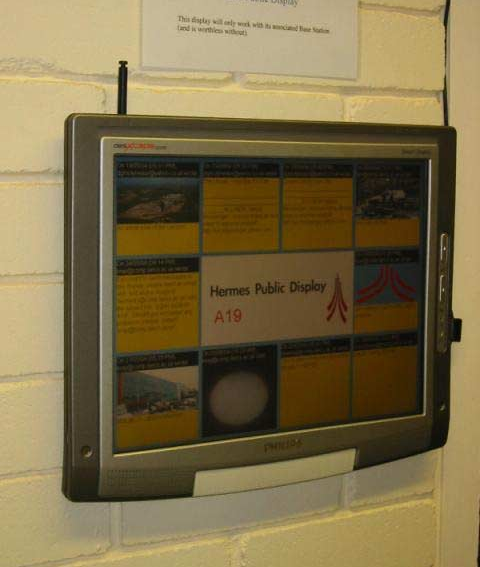
\includegraphics[width=0.5\textwidth]{./img/hermes_photoDisplay_short.png}
  \caption{Das erste Hermes Foto-Display\cite{cheverest:2012}}
  \label{img:hermesPhotoDisplay}
\end{figure}
\\
Um das Hermes System zu erweitern wurde später ein Foto-Display \abb{img:hermesPhotoDisplay} entwickelt\cite{cheveres:2005:hermes-bluetooth}. Da die Hermes-Displays sehr klein waren wurde dieses Display ausschließlich für Bilder verwendet.
Mit dieser Erweiterung war es den Nutzern möglich Bilder per MMS oder Bluetooth an das Gerät zu schicken oder mit der vorhandenen Displaykamera ein Bild zu schießen.
\\
%\todotext{übergang}\\
\\
Da dieses System schon 2003 entwickelt wurde, dienten dessen Ausarbeitungen und Forschungsergebnisse als Inspiration oder Grundlage für andere Projekte, wie \bspw für das NetBoards System. 

\section{NetBoards}
NetBoards\cite{wood:2014,netboards:website} ist ein weiteres interessantes Projekt im Bereich interaktiver digitaler Türschilder. Es wurde 2014 an der Universität von Camebridge entwickelt und zielte darauf ab \quelle{die bereits vorhandenen Whiteboards und Pinnwände neben den Universitätsbüros mit großen, touch-fähigen Bildschirmen zu erweitern oder zu ersetzen}{wood:2014}.
\\
Im Vergleich zum Hermes System hatte sich einiges bezüglich Hardware geändert. \quelle{Displays sind billiger, größer, hochauflösender und energieeffizienter geworden}{wood:2014}.
Dadurch konnten für NetBoards größere Bildschirme mit höherer Auflösung \abb{img:netBoardsDisplay} verwendet werden als beim Hermes System.
\begin{figure}[h!]
  \centering
    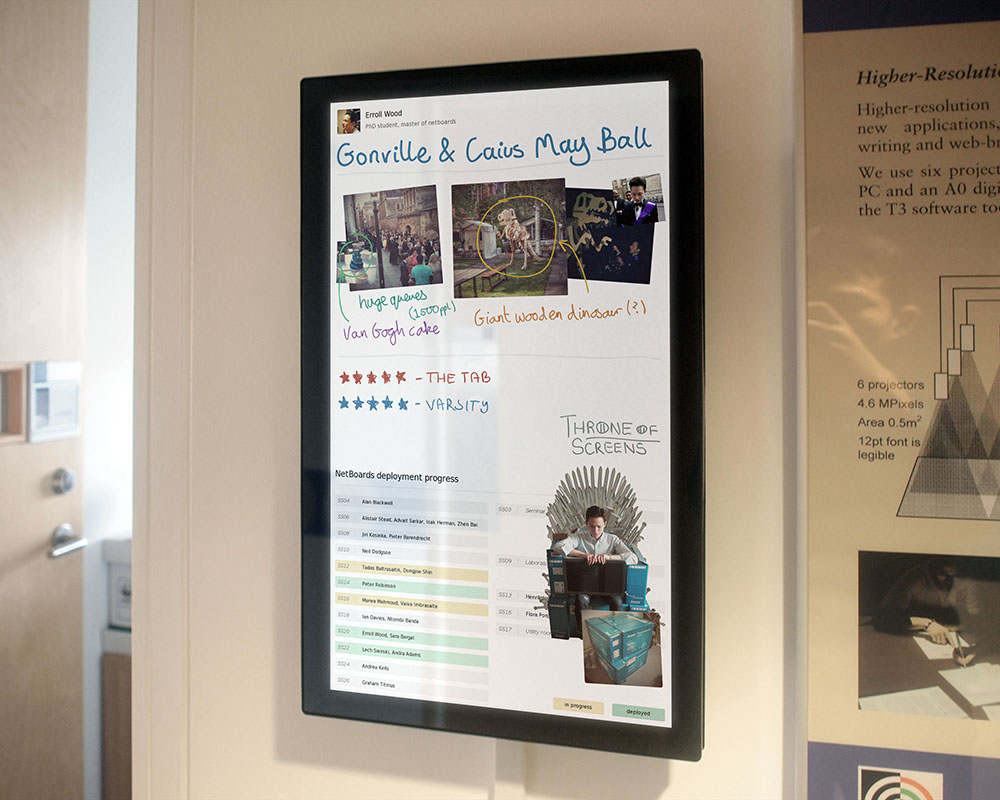
\includegraphics[width=0.7\textwidth]{./img/netBoards_display.png}
  \caption{Das NetBoards Display\cite{wood:2014}}
  \label{img:netBoardsDisplay}
\end{figure}
\\
% Prototyp Entwicklung
Die ersten Prototypen des NetBoard Systems bestanden jeweils aus einem 22 Zoll großem Touchscreen-Monitor, der von einem Raspberry Pi\footnote{Ein Raspberry Pi ist ein kompakter Einplatinencomputer \cite{raspberrypi:website}} betrieben wurde.
Im ersten Experiment der Entwickler wurden fünf Prototypen verwendet, um herauszufinden, ob die Boards akzeptiert werden und um typische Nutzerverhalten zu bestimmen.
\quelle{Diese wurden vor den Büros von Doktoranden, Post-Doktoranden und eines Professors aufgehängt, um herauszufinden, wie diese unterschiedlichen Mitarbeiter mit dem System umgehen würden}{wood:2014}
\quelle{Die Probanden konnten bei diesem Experiment Skizzen und Nachrichten zeichnen sowie Bilder per Web-Interface hochladen}{wood:2014}. Zudem war es möglich, Webseiten zu laden, die dann in einer Hintergrundschicht angezeigt werden konnten.
\\
Während des Experiments fanden die Entwickler heraus, dass die Boards schnell Aufmerksamkeit erzeugten. \quelle{Vorbeigehende Leute begannen spontan mit den Bildschirmen zu interagieren oder sogar die Besitzer direkt auf die Boards anzusprechen}{wood:2014}.
Als Ergebnis des Experiments zeigte sich, dass zwei wichtige Faktoren die Akzeptanz der Nutzer gegenüber den Boards beeinflussten:
%Dependability = Zuverlässigkeit
%Ease of use = Benutzerfreundlichkeit
\begin{itemize}
  \item \textbf{Zuverlässigkeit}: \quelle{Nutzer werden ein System nur benutzen wenn sie denken es funktioniert}{wood:2014}
  \item \textbf{Benutzerfreundlichkeit}: \quelle{Angewöhnung der Nutzer an das System ist unwahrscheinlich, wenn das System schwer zu benutzen ist oder es zu viel Übung erfordert}{wood:2014}
\end{itemize}
Da für die Prototypen Touchscreens mit SAW-Technologie\footnote{Surface-Accoustic-Wave (dt.: Akkustische Oberflächenwelle) ist eine Technik um die Position von Fingern auf Displays zu ermitteln.} eingesetzt wurden, war die Interaktion mit den Boards sehr ungenau, wodurch die Benutzerfreundlichkeit stark beeinträchtigt wurde.
Zudem waren die Raspberry Pi's zu schwach, um ein funktionsreiches Interface zu betreiben.
\\
\\
Nach dem Experiment passten die Entwickler ihr System an.
Sie ersetzten die Raspberry's mit leistungsfähigeren Maschinen, die jeweils in der Lage waren zwei Monitore simultan anzusprechen.
Um es von überall erreichen zu können wurde das NetBoards-System mit Web-Technologien implementiert. \quelle{Es musste möglich sein, mit mobilen Telefonen oder Tablet-PC's das System zu erreichen}{wood:2014}.
Der Server bestand deswegen aus einem einfachen Webserver, der beim Aufruf eine HTML Webseite auslieferte. Frontend Funktionen wurden per Javascript realisiert, wobei die Ansicht der Displays in drei Schichten aufgeteilt wurde\cite{wood:2014}:
\begin{itemize}
  \item \textbf{UI (Benutzerinterface)}\\
    für Interface Widgets\footnote{\todo} und Details über die Bewohner des Büros
  \item \textbf{Board Content (Board-Inhalt)}\\
    für gezeichnete Nachrichten, Skizzen und Bilder
  \item \textbf{Web-Page Background (Hintergrund Webseite)}\\
    zur Anzeige einer beliebigen Webseite
\end{itemize}
Mit diesen neuen Spezifikationen wurde ein Testlauf über mehrere Monate durchgeführt. \quelle{Die Boards erzeugten in diesem neuen Test erhöhte Aufmerksamkeit und die Besitzer nutzten sie mehr, um ihre Kollegen von ihren Abwesenheiten zu informieren, selbst wenn sie nicht persönlich vor Ort waren}{wood:2014}. \quelle{Im ersten Test änderten die Nutzer nur den Inhalt ihres eigenen Boards, was sich im zweiten Test änderte. Sie begannen auch den Inhalt der Boards ihrer Kollegen zu ändern.}{wood:2014}
\\
%\todotext{übergang}\\
\\
Da NetBoards eines der neuesten Systeme für interaktive Türschilder ist, flossen in die Ausarbeitung Teile von früheren Forschungen ein, unter anderem aus dem Hermes System, aber auch von diversen anderen Projekten.


\section{Andere}
%%%%%%%%%%%%%%%%%%%%%%%%%%%%%%%%%%%%%%%%%%%%%%%%%%%%%%%%%%%%%%%%%%%%%%%%%%%%%%%%
%Florian-Note: (DONE)
%Das würde ich etwas ausführlicher machen, nicht nur Bullet points. Vielleicht einfach nur jeweils noch einen Satz, wie sich das von den vorigen Systemen unterscheidet.
%%%%%%%%%%%%%%%%%%%%%%%%%%%%%%%%%%%%%%%%%%%%%%%%%%%%%%%%%%%%%%%%%%%%%%%%%%%%%%%%
Diese anderen wissenschaftlich Arbeiten befassen sich teilweise mit dem Konzept von interaktiven Türschildern oder wurden nur theoretisch erarbeitet.
\\\\
Im wissenschaftlichen Paper ``Dynamic Door Displays'' von David Nguyen et al. ging es darum, eine Möglichkeit zu entwickeln, um die natürlichen Anzeigefähigkeiten von Bürotüren zu erweitern. Dies umfasste automatische Updates und maßgeschneiderte Displays zur Präsentation von privaten Informationen\cite{nguyen:dyn-door-disp}. Die Ausarbeitung ähnelte in gewisser Hinsicht dem Hermes-System, nur das anstelle eines PDA's ein Hewlett-Packard 620LX Handheld-Computer zum Einsatz kam.
Leider wurde nur ein Prototyp entwickelt, das System danach aber nicht weiter geführt. Jedoch bot dieses Projekt einige Grundlagen für Hermes, sowie NetBoards.
\\\\
In der Arbeit ``Semi Public Displays for Small, Co-located Groups'' von Elaine M. Huang et al. ging es um Displays in halb öffentlichen Räumen. \quelle{Das System beinhaltete die Bereitstellung von Informationen an abgeschiedenen Orten oder für Leute, die keine Kenntnis über die Arbeiten ihrer Kollegen haben.}{huang:2003} Es bot mehrere untereinander unabhängige Funktionen für die Darstellung und Interaktion auf peripheren Displays an. Im NetBoards Projekt wurde jedoch entschieden, Funktionen zusammenzuführen, wodurch \bspw die Anzeige einer statischen Webseite mit der Funktion eines Editors für Skizzen verbunden wurde.
\\\\
Die wissenschaftliche Ausarbeitung ``UniCast, OutCast \& GroupCast: Three Steps Toward Ubiquitous, Peripheral Displays'' von Joseph F. McCarthy et al. handelt von drei verschiedenen Display-Varianten: OutCast - Display außerhalb eines Büros, UniCast - Display in einem Büro und GroupCast - Display in einem Gemeinschaftsbereich\cite{mccarthy:2001}. Die OutCast Displays sind eine weitere Variante von interaktiven Türschildern im Bürobereich. Sie wurden dazu genutzt um Biographien, Kalender-, Positions-, Projektinformationen, Demonstrationen oder Textnachrichten anzeigen zu lassen. Dieses Projekt war eines der ersten Systeme für die Anbringung von Bildschirmen außerhalb von Büros zur Informationsdarbietung. Deshalb hatte es auch gewissen Einfluss auf die späteren Entwicklungen.